\documentclass{report}
\usepackage[utf8]{inputenc}

\usepackage{listings}

\usepackage{subcaption}
\usepackage{hyperref}
\usepackage{latexsym}
\usepackage{amssymb}
\usepackage{amsmath}
\usepackage{mnsymbol}
\usepackage{graphicx}
\usepackage[titletoc]{appendix}
\usepackage{comment}

\usepackage{incgraph}
\usepackage{tikz}
\usetikzlibrary{positioning}
\usetikzlibrary{shapes.geometric, arrows}

\tikzset{
  blueNode/.style={circle,
    draw=blue!60, fill=blue!20,
    thick},
  redNode/.style={circle,
    draw=red!60, fill=red!20,
    thick}}
\makeatletter
\tikzset{selfloop/.style =  {to path={
      \pgfextra{\let\tikztotarget=\tikztostart}
      [min distance=7mm]
      \tikz@to@curve@path},font=\sffamily\small
  }}  
\makeatletter

\usepackage{cleveref}[noabbrev]

\crefname{equation}{}{}  
\Crefname{equation}{}{}

\usepackage{xcolor}
\newcommand\questions[1]{\textcolor{red}{#1}}

\definecolor{codegreen}{rgb}{0,0.6,0}
\definecolor{codegray}{rgb}{0.5,0.5,0.5}
\definecolor{codepurple}{rgb}{0.58,0,0.82}
\definecolor{backcolour}{rgb}{0.95,0.95,0.92}

\lstdefinestyle{mystyle}{
  backgroundcolor=\color{backcolour},   
  commentstyle=\color{codegreen},
  keywordstyle=\color{magenta},
  numberstyle=\tiny\color{codegray},
  stringstyle=\color{codepurple},
  basicstyle=\ttfamily\footnotesize,
  breakatwhitespace=false,         
  breaklines=true,                 
  captionpos=b,                    
  keepspaces=true,                 
  numbers=left,                    
  numbersep=5pt,                  
  showspaces=false,                
  showstringspaces=false,
  showtabs=false,                  
  tabsize=2
}

\lstset{style=mystyle}

\title{Model Checking Report: Assignment 2}
\author{Massimiliano Mirelli\footnote{A1.2} \\  \href{mailto:s202339@dtu.dk}{s202339} \and Mehmet Mert Yozdamar\footnote{A2.2} \\ \href{mailto:s183417@dtu.dk }{s183417} }

\date{\today}
\begin{document}

\maketitle
\tableofcontents
\newpage

\part{Part A: Introductory problems}

\chapter{Part A1: Practical Problems}
\begin{enumerate}
\item
  \begin{enumerate}
  \item The non-deterministic actions happen both locally and due to concurrency. Specifically, the actions labelled \verb|createi| are non-deterministic, locally in \verb|clienti| and due to concurrency in \verb|scheduler|. In the former case, this happens since the guards are all satisfied at the program start; in the latter as both clients could be starting at the same time in a state where \verb|create1| and \verb|create2| labelled actions are to be executed. 
  \item The modules non-deterministic (\verb|create|) actions have been modified as instructed using the uniform distribution:
    \begin{itemize}
    \item $p=0.2$ for \verb|clienti|;
    \item $p=0.5$ for \verb|scheduler|;
    \end{itemize}  
    see \Cref{mod:FCFS-DTMC} for more details.
  \item 83 states.
  \item The concurrent non-determinism was eliminated using only one action \verb|create| instead of having two (\verb|createi|). Additionally, we assigned equal probabilities to the updates of the \verb|create|-labelled action in \verb|scheduler|.
  \item In order for the property to be satisfied, we needed to assign both positions of the queue to one client in the \verb|scheduler|'s \verb|create| action.
  \end{enumerate}
\item
  \begin{enumerate}
  \item From the results in \Cref{res:FCFS-DTMC-ss}, we have observed that the only state having an empty queue is the first one. Thus the probability that there are no jobs in the queue is equal to the probability of the DTMC being in that state ($0.10000012259438058$).
  \item We have used the weighted average in \cref{eq:form-A1-2} to approximate the expected length of \verb|client1| jobs. In this case, we consider the steady state probabilities ($p_{i}$) for an active state (i.e. a state where $\mathtt{task1}=1$) to be the weights, and the possible job lengths ($\ell_{i}$) the data elements. Thus, $n$ is the number of states for which $task1 = 1$ holds.
    \begin{equation}
      \label{eq:form-A1-2}
      \frac{ \sum_{i=1}^{n}p_{i}a_{i} \ell_{i}}{ \sum_{i=1}^{n}p_{i}a_{i}}
    \end{equation}
    Based on the final result, $2.230769332929036$, we can conclude that the expected number of tasks in a job is $2$. This was computed utilising \Cref{test:a12b}.
  \item The probability that \verb|client1| does not have a job at time 10 is equal to the probability of the DTMC of being in a state in which $\mathtt{task1} = 0$ holds. This occurs in the first 18 states of \Cref{res:FCFS-DTMC-t10}, hence the sum of the corresponding probabilities (0.5200000000000002 - computed by \Cref{test:a12c}) is the answer to the question.
  \item \Cref{fig:a12d}  shows that \verb|client1| queue becomes full at time $t=1$ (after being empty at time $t=0$), as it gets completely busy after \texttt{create} action is executed. When $t>2$, the number of states where the queue is freed progressively increases, as tasks are handled by \texttt{scheduler} (as in the state \texttt{(s1=1,t1=1,...)} becoming \texttt{(s1=1,t1=0,...)} at $t=2$). Finally, at times $t \in \{9,10\}$, the number of states with \texttt{job1} empty decreases as new tasks are generated by \texttt{client1} and this hints that the probability tends to a constant value, for $n \rightarrow \infty$.
    \begin{figure}[h]
      \begin{center}
        \includegraphics[width=.7\textwidth]{./code/results/a12d-plot.png}
        \caption{Transient probability up to time 10 of the event "Client1 has no jobs active", plotted using \Cref{test:FCFS-DTMC-t10-plot}}
        \label{fig:a12d}
      \end{center}
    \end{figure}
  \end{enumerate}
\item
  \begin{enumerate}
  \item \cref{log:A13a} is satisfied by the initial state of \Cref{mod:FCFS-DTMC}.
    \begin{gather} \label{log:A13a}
      \texttt{P>0.2 [ X (state1 = 1 \& task1 > 2) ]} 
    \end{gather}
  \item \cref{log:A13b} is satisfied by the initial state of \Cref{mod:FCFS-DTMC}.
    \begin{gather} \label{log:A13b}
      \texttt{P<0.5 [ F <= 10 (task2 = 5) ]} 
    \end{gather}
  \item \cref{log:A13c} is not satisfied by the initial state of \Cref{mod:FCFS-DTMC}.
    \begin{gather} \label{log:A13c}
      \texttt{P>0 [ G (task1 > 0) ]} 
    \end{gather}
  \item The probability values of the above properties holding of the initial state in the model (\Cref{mod:FCFS-DTMC}) are respectively:
    \begin{enumerate}
    \item 0.60, for \cref{log:A13a};
    \item 0.28, for \cref{log:A13b};
    \item 0.00, for \cref{log:A13c}.  
    \end{enumerate}
  \end{enumerate}
  \item
    \begin{enumerate}
    \item Given a DTMC $\mathcal{M}:=(S, \mathbf{P}, \iota_{init}, AP, L)$ the induced TS $\mathcal{T}(\mathcal{M}) := (S, Act, \rightarrow, I, AP, L)$ where
      \begin{itemize}
      \item $Act := \{ \tau \}$, where $\tau$ is an action placeholder;
      \item $\rightarrow := \{(s,\tau,s') \in S \times Act \times S \ \vert \ \mathbf{P}(s,s') > 0 \}$
      \item $I := \{ s_{i} \ \vert \ \iota_{init}(s_{i}) > 0 \}$
      \end{itemize}
      If $\Phi$ is a CTL formula, we say that $\mathcal{M} \models \Phi \quad \text{iff} \quad \mathcal{T}(\mathcal{M}) \models \Phi$.

    \item Given the DTMC $\mathcal{D}_{0}$ (\Cref{fig:A14b-dtmc}), and the induced TS $\mathcal{T}(\mathcal{D}_{0})$ (\Cref{fig:A14b-ts}). We observe that $\mathcal{D}_{0} \models \neg P_{\leq 0}(G \Phi)$ but $\mathcal{D}_{0} \nmodels \Psi:= E\ G\ \Phi \ \text{as} \ \mathcal{T}(\mathcal{D}_{0}) \nmodels \Psi$.

      \begin{figure}[h!]
      \centering
      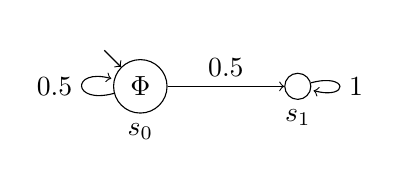
\begin{tikzpicture}[->,main/.style = {draw, circle},node distance=2cm and 4cm]
        \node[main,label=below:$s_0$] (1) {$\Phi$};
        \node[main, above left=.3cm of 1,draw=none] (0) {};
        \node[main,label=below:$s_1$] (2) [right of=1] {};
        \path[]
        (0) edge node [] {} (1)
        (1) edge[loop left] node [] {0.5} (1)
        (1) edge node [above] {0.5} (2)
        (2) edge[loop right] node [] {1} (2);
      \end{tikzpicture}
      \caption{$\mathcal{D}_{0}$ DTMC - Exercise A1.4b)} \label{fig:A14b-dtmc}
    \end{figure}

      \begin{figure}[h!]
      \centering
      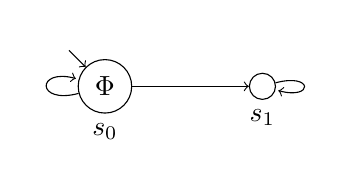
\begin{tikzpicture}[->,main/.style = {draw, circle},node distance=2cm and 4cm]
        \node[main,label=below:$s_0$] (1) {$\Phi$};
        \node[main, above left=.3cm of 1,draw=none] (0) {};
        \node[main,label=below:$s_1$] (2) [right of=1] {};
        \path[]
        (0) edge node [] {} (1)
        (1) edge[loop left] node [] {} (1)
        (1) edge node [above] {} (2)
        (2) edge[loop right] node [] {} (2);
      \end{tikzpicture}
      \caption{$\mathcal{T}(\mathcal{D}_{0})$ TS - Exercise A1.4b)} \label{fig:A14b-ts}
    \end{figure}
  \item This is the case as $\Theta_{n}(s_{1}) \xrightarrow[]{n \rightarrow \infty}1 $ for  $\mathcal{D}_{0}$. In other words, the DTMC will keep being in $s_{0}$ with a very low probability.
    \item The fact that a TS satisfying a CTL formula can execute the same transition for an unlimited number of times, as no the model transitions are not bound to any probability distribution. Hence, non-determinism is the element which PCTL does not manage to capture.
  \end{enumerate}
\end{enumerate}

\chapter{Part A2: Theoretical Problems}

\chapter{Part B1: Practical Problems}

For our basic pre-emptive lottery scheduler (in \Cref{mod:LS-b11a}), we decided to model the tickets with an integer variable per client (\texttt{ti}). Below, we describe the semantics of \texttt{ti} domain:

\begin{itemize}
\item 1 : (i.e. enabled) \texttt{clienti} is allowed to execute a task;
\item 0 : (i.e. unset) \texttt{clienti} is pre-emptied, meaning that, currently, it cannot execute a task;
\item -1 : (i.e. disabled) \texttt{clienti}'s job has just terminated and it will not be allowed to execute a task, until all clients will have executed their current ones.
\end{itemize}

The semantics is enforced by the \texttt{servei} and \texttt{finishi} actions. A property of this model is that at every time at most one ticket is active. This ensures determinism in both executing tasks and finishing jobs. Also, it models the quantum as a time unit, since each time \texttt{clienti}'s task is executed, \texttt{ti} is unset, and similarly when a job is terminated \texttt{ti} is disabled.

Additionally, the model is starvation-free. This is ensured by the \texttt{ti} domain semantics, which prevents a client from getting a job continuously executed. The reason of this is that \texttt{ti} is disabled when \texttt{scheduler} completes \texttt{clienti}'s job and it is enabled again by \Cref{lst:ti-reactivate}, when all other clients' jobs have been executed.

\begin{lstlisting}[caption=Action in enabling ti back - from \Cref{mod:LS-b11a},label=lst:ti-reactivate]
[] t1=-1 & t2=-1 & t3=-1 -> 1: (t1'=0) & (t2'=0) & (t3'=0);
\end{lstlisting}

\begin{equation}
  \label{eq:phi-b11}
  \Phi: \text{"}\mathtt{client1} \ \text{completing its first job within T time units"}
\end{equation}


The probability distribution of $\Phi$ \Cref{eq:phi-b11} seems to confirm the fact that every client is eventually handled by the scheduler. \Cref{fig:b11c} shows the probability computed by \Cref{log:b11c}, rising over $0.5$ for $T=20$. The actual numerical results can be verified in \Cref{res:b11c}. 

\begin{lstlisting}[caption=Command to compute probabilities in \Cref{fig:b11c},label={log:b11c}]
  prism LS-b11a.pm -const T=0:20 -pf 'P=?[ F<=T finished=true ]'  -exportresults ../results/LS-b11a.log}
\end{lstlisting}

\begin{figure}[h]
  \begin{center}
    \includegraphics[width=.7\textwidth]{./code/results/b11c.png}
    \caption{Probability of $\Phi$ \Cref{eq:phi-b11}, plotted using \Cref{test:LS-b11c} and data \Cref{res:b11c} produced by \Cref{log:b11c}}
    \label{fig:b11c}
  \end{center}
\end{figure}

It should also be noted the way quantum can be increased to more than one time unit by slightly modifying the domain of \texttt{ti}. In the modified model \Cref{mod:LS-b11e}, \texttt{ti} may also be assigned to value 2, meaning that two operations (either \texttt{servei}*2 or \texttt{servei}+\texttt{finishi}) for \texttt{clienti} will be handled next. As predictable, since more actions per quantum (i.e. higher number of quantums) are granted, the probability distribuition (\Cref{fig:b11e}) grows faster and has an higher maximum than the previous distribution.

\begin{lstlisting}[caption=Command to compute probabilities in \Cref{fig:b11e},label={log:b11e}]
  prism LS-b11e.pm -const T=0:20 -pf 'P=?[ F<=T finished=true ]'  -exportresults ../results/LS-b11e.log}
\end{lstlisting}

\begin{figure}[h]
  \begin{center}
    \includegraphics[width=.7\textwidth]{./code/results/b11e.png}
    \caption{Probability of $\Phi$ \Cref{eq:phi-b11}, plotted using \Cref{test:LS-b11c} and data \Cref{res:b11e} produced by \Cref{log:b11e}}
    \label{fig:b11e}
  \end{center}
\end{figure}

Assigning different number of tickets to each client is another modification we have experimented on the lottery scheduler (\Cref{mod:LS-b12a}). This is modelled by probabilities on unlabelled actions, which are the only significant additions to the previous model. We take \Cref{lst:b12a} as an explanatory example. The example consists of two actions, let us first focus on the second one. In this case, we observe that the distribution of assigning the next processing slot is not uniform, but dependent on the job lengths. Specifically, a \texttt{clienti}'s task is prioritized if the size of the other tasks is large or, equivalently, its task size is small. In other words, we are simulating a Shortest Remaining Time (SRT) scheduler, using the DTMC most significant peculiarity: probabilities. Secondarily, guard and probabilities differ in the \Cref{lst:b12a} actions. In the states where \texttt{task1=0 OR task2=0 OR task3=0} holds, the probability distribuition of assigning the next time slot must be uniform, as there is no way to prioritize using task lengths. \Cref{mod:LS-b12a} contains several other similar actions, all constructed accordingly, in order not to disrupt the previous development. As a result, the number of states of the extended model is equals to the previous one and we can confidently conclude that the two also share the starvation-free property. 

\begin{lstlisting}[caption=Addition to \Cref{mod:LS-b11a} modelling different number of tickets per client,label=lst:b12a]
  [] t1=0 & t2=0 & t3=0 & (task1*task2*task3)=0 -> 1/3: (t1'=1) + 
                                                   1/3: (t2'=1) + 
                                                   1/3: (t3'=1) ;
  [] t1=0 & t2=0 & t3=0 & (task1*task2*task3)!=0 ->
                     (task2+task3)/(2*(task1+task2+task3)):(t1'=1)+ 
                     (task1+task3)/(2*(task1+task2+task3)):(t2'=1)+
                     (task1+task2)/(2*(task1+task2+task3)):(t3'=1);
\end{lstlisting}

The only drawback of model \Cref{mod:LS-b12a} are the hardcoded actions, which make it very difficult (and error-prone) to include more clients to the model. Consequently, we have decided not to add more clients, estimating that the testing environment could support up to 2 more clients, due to the state explosion problem.

Finally, the resistance to DDoS attacks has been tested over the model in \Cref{mod:LS-b12d}. This model extends the one in \Cref{lst:b12a}, by adding new client modules and constant (\texttt{DDoSSize}) to indicate the size of the malicious job. As a result, we managed to model the case when two clients submit jobs of length 1 and the attacker (\texttt{client2}) one of length \texttt{DDoSSize}. A stronger property than $\Phi$\Cref{eq:phi-b11} has been tested by \Cref{log:b12d}. Its result was a constant probability equals to 1.0, hinting that the model is likely to be resistant to DDoS attacks. As a matter of fact, given the PCTL semantics, we are not guaranteed that a property holds of a model. However, we can be reasonably confident that a state where DDoS has negative consequences on the model is fairly rare.

\begin{lstlisting}[caption=Command to compute probabilities in \Cref{fig:b11c},label={log:b12d}]
prism LS-b12d.pm  -const T=0:20,DDoSSize=1000 -pf 'P=?[ G P>=1 [ F finished=true ] ]' -exportresults stdout
\end{lstlisting}

\chapter{Part B2: Theoretical Problems}

\begin{enumerate}
\item
\item See \Cref{fig:b22-1,fig:b22-2,fig:b22-3,fig:b22-4}.

\begin{figure}[p]
    \vspace*{-2cm}
    \makebox[\linewidth]{
        \includegraphics[width=1.3\linewidth]{./fig/b22-1.jpg}
      }
    \caption{Solution to Part B2.2 - 1}
    \label{fig:b22-1}
\end{figure}

\begin{figure}[h]
    \makebox[\linewidth]{
      \includegraphics[width=1.3\textwidth]{./fig/b22-2.jpg}
      }
    \caption{Solution to Part B2.2 - 2}
    \label{fig:b22-2}
\end{figure}

\begin{figure}[h]
    \makebox[\linewidth]{
      \includegraphics[width=1.3\textwidth]{./fig/b22-3.jpg}
    }
    \caption{Solution to Part B2.2 - 3}
    \label{fig:b22-3}
\end{figure}

\begin{figure}[h]
    \makebox[\linewidth]{
      \includegraphics[width=1.3\textwidth]{./fig/b22-4.jpg}
      }
    \caption{Solution to Part B2.2 - 4}
    \label{fig:b22-4}
\end{figure}

\end{enumerate}


\chapter{Part C2: Theoretical Problems}

\begin{figure}[h]
    \makebox[\linewidth]{
      \includegraphics[width=1.3\textwidth]{./fig/c2.jpg}
    }
    \caption{Solution to Part C2}
    \label{fig:c2}
\end{figure}

\begin{appendices}
  \chapter{PRISM Models}
  \lstinputlisting[caption=FCFS-DTMC.pm Solution to A1.1,label={mod:FCFS-DTMC}]{./code/models/FCFS-DTMC.pm}
  \lstinputlisting[caption=LS-b11a.pm Solution to B1.1(a-d),label={mod:LS-b11a}]{./code/models/LS-b11a.pm}
  \lstinputlisting[caption=LS-b11e.pm Solution to B1.1(e),label={mod:LS-b11e}]{./code/models/LS-b11e.pm}
  \lstinputlisting[caption=LS-b12a.pm Solution to B1.2(a-b),label={mod:LS-b12a}]{./code/models/LS-b12a.pm}    
  \lstinputlisting[caption=LS-b12d.pm Solution to B1.2(d),label={mod:LS-b12d}]{./code/models/LS-b12d.pm}  

  \chapter{Results}
  \lstinputlisting[caption=Results of \texttt{prism -ss FCFS-DTMC.pm},label={res:FCFS-DTMC-ss}]{./code/results/FCFS-DTMC_ss.log}
  \lstinputlisting[caption=Results of \texttt{prism -tr 10 FCFS-DTMC.pm},label={res:FCFS-DTMC-t10}]{./code/results/FCFS-DTMC_ss.log}
  \lstinputlisting[caption=Results of \Cref{log:b11c},label={res:b11c}]{./code/results/LS-b11a.log}
  \lstinputlisting[caption=Results of \Cref{log:b11e},label={res:b11e}]{./code/results/LS-b11e.log}    
  
  
  \chapter{Additional tests}
  \lstinputlisting[caption={Python script computing \cref{eq:form-A1-2} and making use of \Cref{res:FCFS-DTMC-ss} },label={test:a12b},language={Python}]{./code/tests/a12.py}
  \lstinputlisting[caption={Python script computing solution to A2.2(c) and making use of \Cref{res:FCFS-DTMC-t10} },label={test:a12c},language={Python}]{./code/tests/a12c.py}    
  \lstinputlisting[caption={Python script computing solution to A2.2(d)},label={test:FCFS-DTMC-t10-plot},language={Python}]{./code/tests/a12d.py}
  \lstinputlisting[caption={Python script plotting graphics for B1.2(c,e), using results in \Cref{res:b11c,res:b11e}},label={test:LS-b11c},language={Python}]{./code/tests/LS-F_T-plot.py}
\end{appendices}

\end{document}

